%% Example file for a masterthesis
% Copyright 2010 by Dirk Willrodt <dwillrodt@zbh.uni-hamburg.de>
% --------------------------------------------------------------
%
% This file may be distributed and/or modified under the
% conditions of the LaTeX Project Public License, either version 1.2
% of this license or (at your option) any later version.
% The latest version of this license is in:
%
%    http://www.latex-project.org/lppl.txt
%
% and version 1.2 or later is part of all distributions of LaTeX
% version 1999/12/01 or later.
%
% Usage: just compile it with pdflatex, and see how it looks, and what caused
% this. You can also take it and change blocks marked like this:
%%%%>
% ...
%%%%<
% to produce Your own thesis.
%
% check chapters in sub folders for examples of usage of different mark-ups


% use the option ger for thesis in german.
% use the option bsc for a bachelor thesis.
% you can pass options to scrreprt, for example numbers=noenddot for if you have
% an appendix and you don't want '.' at the end of chapter numbers
%\documentclass[twoside,a4paper,ger,bsc]{master}
\documentclass[twoside,a4paper,bsc]{master}
%%%%>
% the following package is only needed to produce dummy text.
% You do not need it for your thesis.
\usepackage{lipsum}
% This package is not included in the class, because it is not needed, but we
% recommend to use it. It only works with pdfLaTeX.
\usepackage[kerning,spacing]{microtype}

% add other packages, as needed.
\usepackage{amsmath}
\usepackage{amsfonts}
\usepackage{mathtools}
\usepackage{graphicx}
\usepackage{pdfpages}
\usepackage{algpseudocode}
\usepackage{algorithm}
\usepackage{palatino}
\usepackage{numprint}
\usepackage{svg}
\usepackage{comment}
\usepackage{float}
\usepackage{times}
\usepackage{theorem}
\usepackage{tikz}
\usepackage{amssymb}

\usetikzlibrary{chains}
\usetikzlibrary{decorations.pathmorphing}
\usepgflibrary{decorations.pathreplacing}
\usetikzlibrary{decorations.text}

%%%Comment macro
\newcounter{mycommentcounter}
\newcommand{\Genericcomment}[2]{%
\par%
\noindent%
\fbox{%
\begin{minipage}{0.95\textwidth}
\textsl{#1: \#\refstepcounter{mycommentcounter}%
\arabic{mycommentcounter}: #2}%
\end{minipage}%
}%
\par%
}


\newcommand{\AVTcomment}[1]{
\Genericcomment{AVT}{#1}
}

\newcommand{\SKcomment}[1]{
\Genericcomment{SK}{#1}
}

%%% Other macros
\newcommand{\Qgram}[1]{\(#1\)-gram}
\newcommand{\Query}[0]{\mathsf{Query}}
\newcommand{\Target}[0]{\mathsf{Target}}
\newcommand{\Append}[0]{\mathsf{append}}
\newcommand{\QueryIdx}[0]{\mathsf{QueryIdx}}
\newcommand{\TargetIdx}[0]{\mathsf{TargetIdx}}
\newcommand{\Start}[0]{\mathsf{start}}
\newcommand{\End}[0]{\mathsf{end}}
\newcommand{\TBlockEnd}[0]{\mathsf{TargetBlockEnd}}
\newcommand{\QBlockEnd}[0]{\mathsf{QueryBlockEnd}}
\newcommand{\HashValue}[0]{\mathsf{HashValue}}
\newcommand{\HashValVec}[0]{\mathsf{HashValVec}}
\newcommand{\CurrentWeight}[0]{\mathsf{CurrentWeight}}
\newcommand{\SuffixCode}[0]{\mathsf{SuffixCode}}
\newcommand{\Code}[0]{\mathsf{code}}
\newcommand{\Score}[0]{\mathsf{score}}
\newcommand{\Loopid}[0]{\mathsf{loopid}}
\newcommand{\Wheel}[0]{\mathsf{wheel}}
\newcommand{\IT}[2]{\mathsf{IndexTable}_{#1,#2}}
\newcommand{\LE}[2]{\mathsf{LinearEnc}_{#1,#2}}
\newcommand{\Substring}[3]{#1\lbrack #2\ldots#3\rbrack}
\newcommand{\Subchar}[2]{#1\lbrack #2\rbrack}
\newcommand{\Scoretablename}[0]{\mathsf{ST}}
\newcommand{\Scoretable}[2]{\Scoretablename_{#1}[#2]}
\newcommand{\Reals}{\mathbb{R}}
\newcommand{\Permname}[1]{\varphi_{#1}}
\newcommand{\Perm}[2]{\Permname{#1}(#2)}
\newcommand{\Permnameinverse}[1]{\varphi_{#1}^{-1}}
\newcommand{\Perminverse}[2]{\Permnameinverse{#1}(#2)}
\newcommand{\Alpha}[0]{\mathcal{A}}

\theorembodyfont{\rmfamily}
\theoremheaderfont{\rmfamily\bfseries}
\newcounter{Lemmacounter}
\newtheorem{myLemma}[Lemmacounter]{Lemma}
\newcommand{\AfterNumber}{}
\newcommand{\Skiptheorem}{\smallskipamount}
\newcommand{\StartFormal}[1]{\par\addvspace{\Skiptheorem}\noindent\textbf{#1}}
\newcommand{\EndFormal}{\par\addvspace{\Skiptheorem}}
%\newenvironment{Lemma}{\begin{myLemma}\AfterNumber}{\end{myLemma}}
\newenvironment{Proof}{\StartFormal{Proof:}}{\EndFormal}
\def\FirstMultisetSymbol{\(a_0\)}
\def\SecondMultisetSymbol{\(a_1\)}
\def\ThirdMultisetSymbol{\(a_2\)}

%%%%<

% Helpfull command to put reminders in your work
\newcommand{\Todo}[1]%
{\colorbox{orange}{\mbox{}\\\fbox{\parbox{\textwidth}{\textbf{Todo: #1}}}}\\}
% it uses one argument which is referred to by #1

\newcommand{\Alphabet}{\mathcal{A}\xspace}
\begin{document}

% use roman page numbers before the real document starts.
\pagenumbering{roman}

%Change the values here to get your title page and assertion page right
\AdvisorA{Stefan Kurtz}
\AdvisorB{Andrew Torda}
\author{Anh Viet Ta}
\MatrikelNo{\numprint{6747004}}
%\AuthorAdress{Musterstrasse 1}{07770 M\"unchhausen}
\title{
       \begin{tabular}{c}
       \textbf{Efficient Preprocessing of Short Sequence Segments}\\[3mm]
       \textbf{for Efficient Filtering in Comparing Protein Sequences}
       \end{tabular}}
% add data line or leave it to use current date.
%\date{1.4.2016}
\Maketitle

\SKcomment{Please provide a longer abstract}

% if you write in German, maybe change this to "Zusammenfassung".
\addchap*{Abstract}
\small
%%%%>

The software suite MMseqs2 and its predecessor MMseqs are the new standard
of both sensitive biological sequence searching and sequence clustering.
The prefiltering module in MMseqs2 is of particular importance, since it
serves to rapidly reduce possibility space. This thesis focusses on the
first phase of the filtering approach, i.e.\ the construction of the
\(k\)-environment and shows how to systematically improve its runtime and
space requirement.

%%%%<
\normalsize

% The first sets the depth of the TOC, the second produces it. Change the
% number if you need a ``deeper'' TOC.
\setcounter{tocdepth}{1}
\tableofcontents

%%%%>
% include chapters from subfolders
% change if you need more chapters or if you want to call them different, this
% is just an example

\Chapter{Recent developments of bioinformatic sequence searching and
clustering}

\SKcomment{Use the chapter heading 'Introduction' and the current heading
as section heading. Also MMseqs is not an own chapter, but a section of the
introduction.}
% reset to arabic page numbers will start with 1
\pagenumbering{arabic}
With the advent of high-throughput sequencing technologies, the cost of
sequencing DNA has dramatically be reduced. Sequence databases, such as
UniProt have been growing by a factor of two every two years, which leads
to a significant focus on developing searching and clustering methods that
can handle large-scale datasets efficiently. Algorithms and software that
can scale horizontally (across multiple machines) have gained importance.
On sequence searching, new algorithms and heuristics have been developed to
improve sensitivity without sacrificing speed. Tools like
DIAMOND~\cite{buchfink2015fast} and

\SKcomment{Please  also cite \cite{BUC:REU:DRO:2021} which I added to the
bib file.}

MMseqs2~\cite{steinegger2017mmseqs2} provide fast and sensitive sequence
searching capabilities,
especially in metagenomics and large-scale sequencing projects. Hidden
Markov Model based
methods, such as the HMMER~\cite{finn2011hmmer} software, have been
enhanced to improve their
sensitivity and accuracy, making them invaluable for protein domain and
family searching. The existing algorithms like BLAST have also seen massive
improvement by using GPU parallelization~\cite{vouzis2011gpu} and specific
hardwares, namely
FPGAs (Field-Programmable Gate Arrays)~\cite{guo2012systolic} have been
customized for
accelerating sequence searching algorithms.
Recent developments on metagenomics have also given ways to specialized
databases and algorithms. These databases contain sequences from
environmental samples and enable the identification of novel organisms and
genes within complex microbial communities.
On sequence clustering, myriads of methods have been developed. Graph-based
clustering methods, such as Markov Clustering
(MCL)~\cite{shih2012identifying} and the
Louvain~\cite{rahiminejad2019topological} algorithm,
have gained popularity. These methods model sequences as nodes in a graph
and use edge weights to represent similarities, allowing for the detection
of densely connected clusters within the graph. Density-based methods like
DBSCAN~\cite{ester1996density} (Density-Based Spatial Clustering of
Applications with Noise) have
seen applications in bioinformatics~\cite{karim2021deep}. These algorithms
group sequences based on
the density of data points, enabling the discovery of clusters with varying
shapes and sizes. Traditional distance-based clustering algorithms, such as
hierarchical clustering~\cite{lafond2017new} and
k-means~\cite{hussain2011fpga}, have been adapted and optimized for
large biological datasets.
\Chapter{MMseqs2}
MMseqs~\cite{hauser2014mmseqs} (Many-against-Many sequence searching) is a
software suite for fast
and deep clustering and searching of large datasets.
It consists of three core modules:
\begin{itemize}
\item a fast and sensitive prefiltering module
that eliminates most non-homologous sequences,
\item a local alignment module based on the Smith-Waterman algorithm
using the ideas and implementation techniques described
in~\cite{Farrar:2007hs,ZHA:LEE:GAR:MAR:2013},

\SKcomment{Please check if this is already true for MMseqs.}
\item and a clustering module based on a
similary graph.
\end{itemize}
Due to the modularity of the structure, it allows users to
create workflows tailored to specific clustering and searching needs. The
default workflow utilizes the UniProt databases to create predefined
parameters and resembles the average use case. The second, cascaded
clustering, clusters the input database in multiple steps, increasing the
sensitivity between each steps and therefore enables finding
best-hit-searches 4-10 times faster.

\SKcomment{faster compared to what?}

The third workflow simply compares
databases using only prefiltering and aligning modules. The last workflow
updates clustering between new and old clustered database by deleting
deprecated sequences and appending new sequences to each cluster.
In benchmarks, MMseqs showed to be 4-30 times faster than UBLAST and
RAPsearch2.

\SKcomment{Add citation for UBLAST and RAPsearch2.}

MMseqs could cluster large databases down to 30\% sequence
identity \numprint{2000} times faster than BLASTclust.
An improved, updated version MMseqs2~\cite{steinegger2017mmseqs2} was
published in 2017.

\SKcomment{Do not use \textbackslash{numprint} for years.}

It provides dramatic improvements in both efficiency and sensitivity by
introducing several novel ideas. It revamped the prefiltering stage by
introducing an algorithm to find two consecutive, spaced-seed \Qgram{q} matches
and optimizing memory access. It also allowed the use of \Qgram{7} due to
the speedup of the algorithm. %Need more

\SKcomment{You can just add an item list to mention the most important
improvements.}

An in-depth look into the three core modules is presented below.

\SKcomment{I will skip reading the next section.}

\section{Fast \Qgram{q} prefiltering stage}
In MMseqs, the prefiltering stage is the first step to process all
sequences and serves to reduce the search space significantly, therefore
it's imperative for the algorithm to be as efficient as possible. The
process consists of 4 loops as outlined in
Figure~\ref{fig:prefilterMMseqs}. In the first loop, query sequences are
searched one by one against the target set. For each spaced seed window in
the query sequence (loop 2), a \Qgram{q} is extracted and a list of all
similar \Qgram{q}s with a Blosum62 similarity above a threshold score is
created using a linear-time branch-and-bound algorithm. Lower threshold
scores result in higher average numbers of similar k-mers and thereby
higher sensitivity and lower speed. Each generated \Qgram{q} (loop 3) then
gets queried against a precomputed database of \Qgram{q}s in target
sequences. The sum of scores of the corresponding target sequences then
gets collected in a vector based on the prefiltering score. In the last
step the target score vector is sorted and the best matches get processed
further.
\begin{figure}[t]
\begin{center}
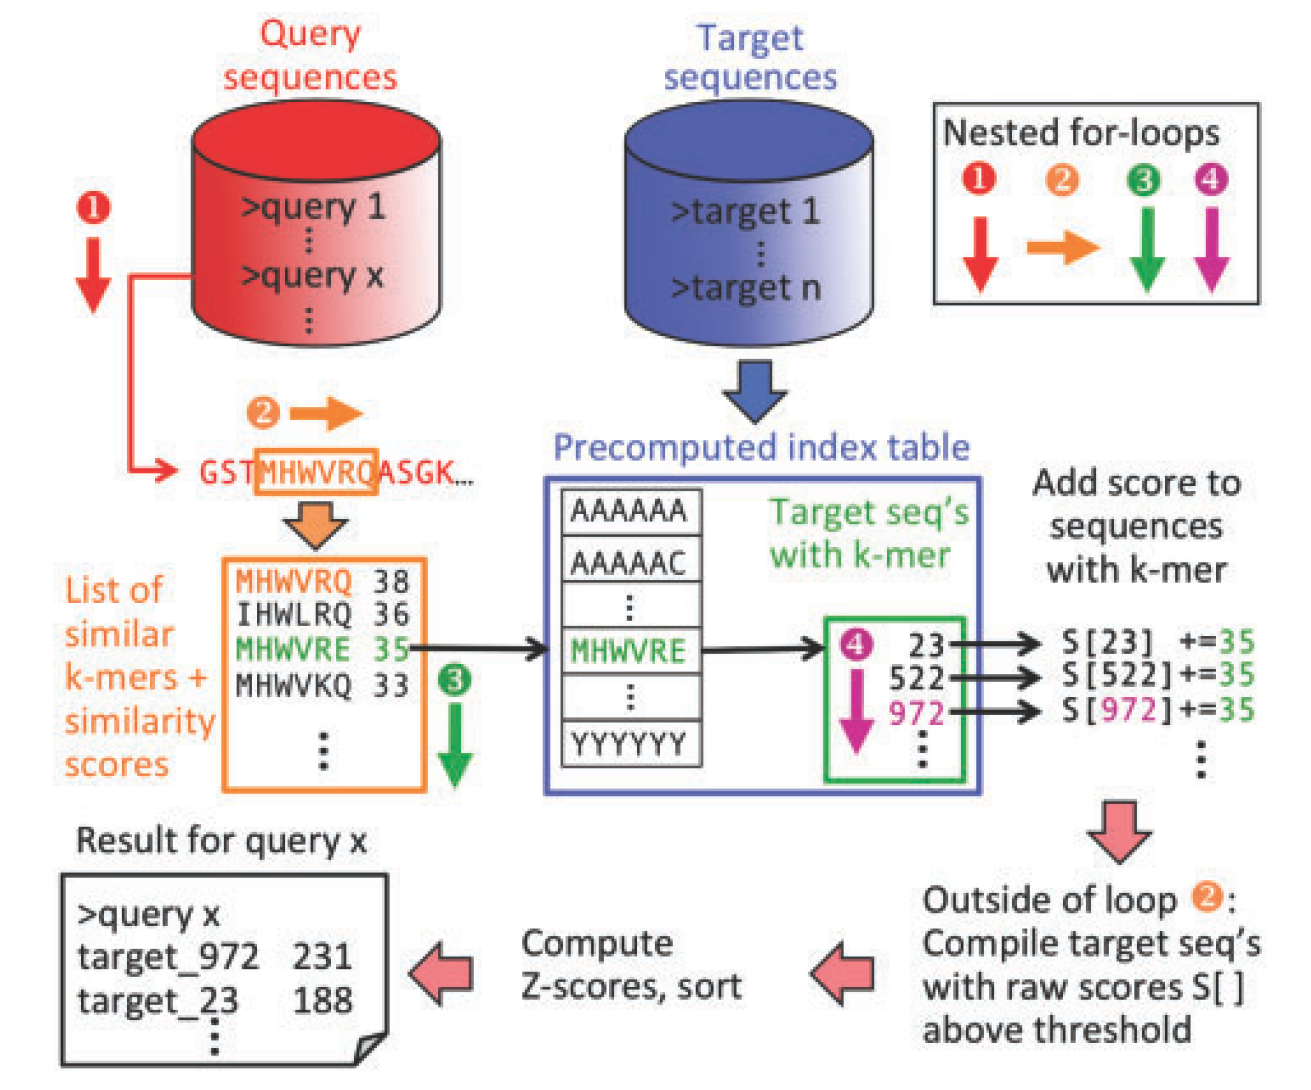
\includegraphics[scale=0.3]{graphics/MMseqs_prefilter.png}
\end{center}
\caption{Prefiltering stage in MMseqs~\cite{hauser2014mmseqs}}
\label{fig:prefilterMMseqs}
\end{figure}
In MMseqs2, the prefiltering stage was reengineered (See
Figure~\ref{fig:prefilterMMseqs2}). After the query-target matches are
collected, they get sorted and iterated over to detect double k-mer matches
by comparing the current diagonal with the previously matched diagonal. If
the previous and current diagonals agree, they both get stored as a double
match for the ungapped alignment stage.
\begin{figure}[t]
\begin{center}
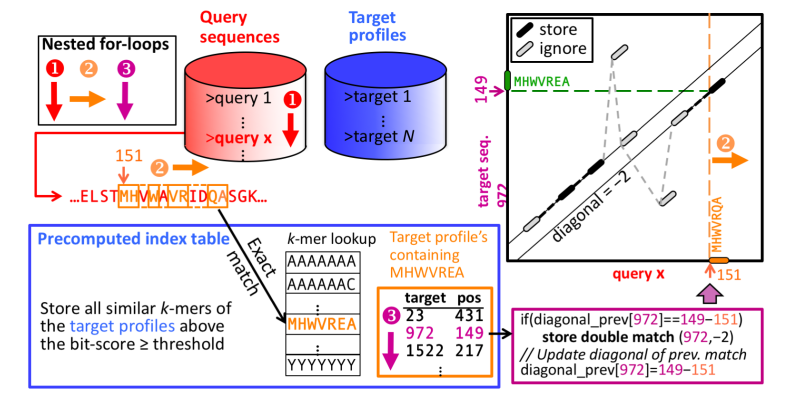
\includegraphics[scale=0.7]{graphics/MMseqs2_prefilter.png}
\end{center}
\caption{Prefiltering stage in MMseqs2~\cite{steinegger2017mmseqs2}}
\label{fig:prefilterMMseqs2}
\end{figure}
\section{Ungapped alignment and Smith-Waterman alignment stage}
In MMseqs2, an additional ungapped alignment stage was introduced, where
many target sequences are aligned at once using a vectorized approach. It
also utilizes a linear memory access using a score matrix containing the p.
Due to the extensive use of SIMD instructions, this stage achieves a linear
time complexity, much more efficient compared to the Smith-Waterman
alignment stage.
After the ungapped alignment is completed, MMseqs2 computes for all
filtered
query-target sequence pairs an exact, unbounded Smith-Waterman alignments
with affine gap penalties. This module utilizes a highly vectorized
algorithm
equipped with new SIMD instructions and adapted for sequence profiles.
\Chapter{Theoretical background}

\SKcomment{This chapter should be named Methods.}
Since for every alphabet \(\Alpha\), a transformer function \(f:\Alpha
\rightarrow \mathcal{N}\) can be defined, mapping every character in
\(\Alpha\) to a integer rank, the following sections will discuss the
biological sequences not as sequences of residues, but as of transformed,
coded integers. The alphabet will also be interpreted mostly as an integer
subset \([0,|\mathcal{A}|)\cap \mathcal{N}\).
\section{Optimizing target data processing}
Since the target database can be very large, a precise and efficient
evaluation must be prioritized. In MMseqs2, at every residue position,
relevant characters based on the user-chosen spaced seed are individually
extracted from the target sequence to create a \Qgram{q}s and then process
these \Qgram{q}s as independent strings. This approach would incur a time
complexity of \(O(q)\) to compute a hash value for each \Qgram{q} and for
the complete sequence of length \(n\) this would sum up to
$O((n-q+1)q)=O(nq)$.
But the \Qgram{q}s are in fact not independent from each other. To create
the next \Qgram{q}, one would only have to remove the first character of
the previous \Qgram{q} and append the next character in the sequence.
Assuming these operations are of constant time complexity, the whole
process would require only $O(n+q)$ time.
This family of hashing algorithms allows efficiently enumerate hash values
of all \Qgram{q}s of a sequence~\cite{cohen1997recursive}. In order to
achieve independence between
hash values, the characters are usually assigned a weight, which might be
expressed as $r^{q-1-i}$, where $r$, the radix, is a constant integer and
$i$ is the position of the character in the \Qgram{q}. The calculation of a
hash value from a \Qgram{q} \(w\) could then be expressed as follows:
\begin{align}
H(w) = \sum_{i=0}^{q-1}r^{q-1-i}w[i]\label{DefineHfunction}
\end{align}
where $w$ is a \Qgram{q} and \(w[i]\) is the \(i\)-th character in \(w\).
As a base case of the recursive algorithm, the hash value for the
first \Qgram{q} of the sequence is computed in \(O(k)\) time by evaluating
the sum defined in Equation (\ref{DefineHfunction}).
Provided we have calculated the hash value of the previous \Qgram{q}
\(ax\), where \(a\) is a character and \(x\) is a \Qgram{q-1}.
Then the hash value
of the next \Qgram{q} could be computed from \(H(ax)\) and the next not yet
processed character, say \(c\). Firstly, the contribution of \(a\)
character is subtracted from the hash value. The virtual window is then
shifted right one character. This means that the weight of all characters
in \(x\) increases by a factor or \(r\). That is, we multiply by the radix.
Lastly, the new character \(c\) is added to the hash.
The hash value of \(xc\) is then calculated as follows:
\begin{align}
H(xc) = (H(ax)-r^{n-1}\cdot a)\cdot r+c\label{IncrementallyComputeH}
\end{align}
Equations (\ref{DefineHfunction}) and (\ref{IncrementallyComputeH})
provide the basic schema of recursive hashing. In implementation, the most
basic form of the algorithm, called invertible integer encoding, is used,
where \(r=|\Alpha|\). The pseudocode for this schema is
outlined in Algorithm \ref{code:invint}.
\begin{algorithm}[t]
\caption{Invertible Integer Encoding}
\label{code:invint}
\begin{tabular}{@{}l@{~}l}
\textbf{Input:}&Encoded sequence $s$ of length $n$\\
&alphabet size \(r=|\mathcal{A}|\)\\
\end{tabular}
\begin{algorithmic}
\State \(\HashValVec\gets []\)
\State \(\HashValue \gets 0\)
\For{\(i\) \textbf{from} 1 to $k$}\Comment{Compute 1st hash}
\State \(\HashValue \gets \HashValue \cdot r\)
\State \(\HashValue \gets \HashValue + s[i]\)
\EndFor
\State \(\HashValVec .\Append(\HashValue)\)
\For{\(j\) \textbf{from} 1 to $n-k$}\Comment{Compute other hash values}
\State \(\HashValue \gets \HashValue - r^{n-1}\cdot s[j]\)
\State \(\HashValue \gets \HashValue \cdot r\)
\State \(\HashValue \gets \HashValue + s[j+k]\)\
\State \(\HashValVec .\Append(\HashValue)\)
\EndFor
\end{algorithmic}
\end{algorithm}
In order to extend the schema to allow for spaced seeds, one could divide
the seed into shorter blocks of \Qgram{q}s, intertwined by blocks of
"Don't Care". Each block can then be treated as individual \Qgram{q} with
custom radix, and the complexity is then \(O(nb)\), where \(b\) is the
number of blocks. Since the number of blocks is in worst case the weight
itself, and in best case 1, recursive hashing has a same or faster time
complexity than normal hashing approachs.
\section{Optimizing query data processing}
In order to quantify the similarity between sequences, a scoring function
is often used. They provide quantitative measures for comparing biological
sequences, structures, and interactions, facilitating a deeper
understanding of biological processes and aiding in drug discovery,
evolutionary analysis, and functional genomics research. In sequence
alignment context, these functions often compare pairwise the biological
residues (often nucleotide bases or proteinogenic amino acids). The most
common scoring function is the substitution matrix, often represented as a
matrix of scores indicating the likelihood of one amino acid (or
nucleotide) being replaced by another. The BLOSUM (Blocks Substitution
Matrix) and PAM (Point Accepted Mutation) matrices are examples of
substitution matrices widely used in bioinformatics. The two families of
score matrices can be summarized as a mathematical function:
\begin{align}
\sigma: \mathcal{A} \times \mathcal{A} \rightarrow \mathcal{R}
\end{align}
A positive score between two residues often denotes similarity between them
and a negative score indicates dissimilarity. The score of between two
sequences \(u,v\in \mathcal{A}^q\) can then be defined as follow:
\begin{align}
\sigma(u,v)=\sum_{i=0}^{|u|-1}\sigma(\Subchar{u}{i},\Subchar{v}{i})\label{equation:sequenceScore}
\end{align}
In order to compute the \(k\)-environment for a \Qgram{q} \(u\)
efficiently, MMseqs2 utilizes a branch-and-bound algorithm, where it
decomposes \(u\) to groups of \Qgram{2}s and \Qgram{3}s \(u_i\),
prioritizing \Qgram{3}. For \(q\in \{2,3\}\), a score matrix
\(\Scoretable{q}{u}=\lbrack (v,\sigma(u,v))\mid v\in\Alpha^{q}\rbrack\) is
computed and sorted after the subscores \(\sigma(u,v))\).
The full $k$-environment of a \Qgram{q} \(u\) can then be iterated as a
subset of the cartesian product \(\bigtimes \Scoretable{|u_i|}{u_i}\):
\begin{align}
\text{Env}_k(u) = \{(v,\sigma(u,v))|(v,\sigma(u,v))\in \bigtimes
\Scoretable{|u_i|}{u_i},\sigma(u,v)\geq k\}\label{ScoreTablesCartesian}
\end{align}
The iteration over score matrix row can be prematurely terminated, as soon
as it's no longer feasible to reach the threshold \(k\).
The key to improve over the method outlined in MMseqs2, is the following:
Given a bijective mapping \(\varphi:\{0,1,\ldots,q-1\}\to
\{0,1,\ldots,q-1\}\). For any sequence of length \(q\), we define a
function
\begin{align}
\varphi(u)=\Subchar{u}{\varphi(0)}\Subchar{u}{\varphi(1)}\ldots\Subchar{u}{\varphi(q-1)}
\end{align}
in that, \ \(\varphi\) permutate the residue in \(u\).
\begin{Lemma}
\label{permutationProof}
Given a special permutation \(\Permname{u}\), so that it orders the
characters in \(u\):
\begin{align}
\Subchar{u}{\Perm{u}{i}}\leq\Subchar{u}{\Perm{u}{i+1}}\forall i, 0\leq
i\leq q-2
\end{align}
The resulted \Qgram{q} \(u_s\) from the permutation is called sorted
\Qgram{q} and could be rearranged using the inverse function:
\begin{align}
\Perminverse{u}{\Perm{u}{i}}=i \forall i, 0\leq i\leq q-1 \Leftrightarrow
\Perminverse{u}{\Perm{u}{u}}=u
\end{align}
Then the following property is valid:
Given a \Qgram{q} \(u\), its sorting permutation \(\varphi_u\) and the
mapping \(u[i] = (\varphi_u (u))[j]\):
\begin{align}
\sigma(\Perm{u}{u},\Perm{u}{v}) = \sigma(u,v)
\end{align}
\begin{Proof}
\begin{align}
\sigma(\Perm{u}{u},\Perm{u}{v}) &= \sum_{j=0}^{q-1} \sigma ((\varphi_u
(u))[j], (\varphi_u (v))[j])\label{eq:jPerm}\\
&= \sum_{i=0}^{q-1} \sigma (u[i],v[i])\label{eq:iPerm} \\
&= \sigma(u,v)
\end{align}
The exchange of variable from Equation~\ref{eq:jPerm} to
Equation~\ref{eq:iPerm} is allowed due to the bijective nature of function
\(\sigma\) and the fact that its domain and codomain are identical.
\end{Proof}
\end{Lemma}
The above proof shows that a permutation function applied on both sequences
\(u\) and \(v\)
permutates the characters in the same way and the score between the
unpermutated sequences is equal to the score between the permutated. This
means that the score matrix ST can be computed only for the sorted
\Qgram{q}s, and it would hold all information needed to compute the full
$k$-environment.
The advantage of this approach is the smaller number of sorted \Qgram{q}s
compared to unsorted, leading to a more efficient memory usage and a more
compacted computation of the score matrix. Any overhead caused by the
rearragement of the sorted \Qgram{q}s could be reduced by SIMD
(Single-Instruction Multiple-Data) instructions.
\section{Working with sorted \Qgram{q}s}
\subsubsection{Enumeration}
In mathematics, a set is defined as a collection of items, where every
element occurs exactly once. This definition can be expanded to multisets,
where elements can occur more than once. Applying an order on these
multisets, we can formalize a notion of sorted \Qgram{q}s:
Given an alphabet \(\Alpha\) and a natural number \(q > 0\), a sorted
\Qgram{q} over \(\Alpha\) is a multiset \(M=a_0a_1...a_{q-1}\),
\(a_i\in\mathcal{A}\forall 0\leq i<q\) and \(a_i \leq a_j\forall 0\leq i <
j < q\).
%The number of possible sorted \Qgram{q}s for a given \(\mathcal(A)\) and
\(q\) can be computed as the binomial \(\binom{q+|\mathcal{A}|-1}{q}\). The
proof can be shown with induction:
An index table of sorted \Qgram{q}s can be computed recursively.
Figure~\ref{fig:enumerate} showcases a model of the problem where \(q=5\)
and \(\Alpha=\{a_0,a_1,a_2\}\). If the prefix of length 2 of \(u\) is
fixed, say \(a_0a_1\), the last 3 characters can be iterated as a sorted
\Qgram{q} of size \(5-2=3\) and alphabet \(\Alpha_1 = \{a_1,a_2\}\). This
could be broken down further and generalized.
Given a sorted \Qgram{q} \(u\) where the prefix of \(m\) characters is
sorted and fixed, and \(u[m-1]\) has a rank of \(a_i\) then the task is to
enumerate every \Qgram{q-m}s of alphabet size (\(|\mathcal{A}|-a_i\)).
The induction base case is then sorted unigrams over alphabet \(\Alpha_i =
\{a_j| a_j\in\Alpha \land j\geq i\}\), where there are \(|\Alpha|-i\)
unigrams indexed from \(a_i\) to \(|\Alpha|-1\).
\begin{figure}[t]
\begin{center}
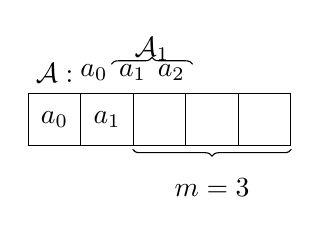
\begin{tikzpicture}
[arraynode/.style={inner sep=1pt,minimum height=19pt,minimum
width=19pt,rectangle,draw},
alphanode/.style={inner sep=1pt,minimum height=15pt,minimum
width=15pt,rectangle},
position label/.style={
below = 3pt,
text height = 1.5ex,
text depth = 1ex
},
overbrace/.style={decoration={brace},decorate},
underbrace/.style={decoration={brace,mirror},decorate}
]
\begin{scope}[start chain=1 going right,node distance=-0.5mm]
\node [alphanode,on chain=1] {\(\mathcal{A}:\)};
\node [alphanode,on chain=1] {\FirstMultisetSymbol};
\node [alphanode,on chain=1] (A0) {\SecondMultisetSymbol};
\node [alphanode,on chain=1] (A1) {\ThirdMultisetSymbol};
\draw [overbrace,decoration={raise=-1ex}] (A0.north west) --
node [position label,yshift=2.5ex] {\(\mathcal{A}_1\)} (A1.north east);
\end{scope}
\begin{scope}[shift={(0cm,-17pt)},start chain=2 going right,node
distance=-0.15mm]
\node [arraynode,on chain=2] {\FirstMultisetSymbol};
\node [arraynode,on chain=2] (Posb) {\SecondMultisetSymbol};
\node [arraynode,on chain=2] (N0) {};
\node [arraynode,on chain=2] {};
\node [arraynode,on chain=2] (N1) {};
\draw [underbrace,decoration={raise=1pt}] (N0.south west) --
node [position label,yshift=-1ex] {\(m=3\)} (N1.south east);
\end{scope}
\end{tikzpicture}
\caption{Example of sorted \Qgram{q}
enumerating\label{fig:enumerate}~\cite{pfn}}
\end{center}
\end{figure}
\begin{algorithm}[t]
\caption{\(\mathsf{MultisetEnumerateRecursion}\)}
\label{code:enumerateMultisetRec}
\begin{tabular}{@{}l@{~}l}
\textbf{Input:}&current multiset length \(q_i\)\\
&current alphabet \(\Alpha_i\)\\
&current prefix \(u\)\\
&current index table \(\IT{q}{\Alpha}\)
\end{tabular}
\begin{algorithmic}
\If{\(q_i = 0\)}
\State \(\IT{q}{\Alpha}.\Append(u)\)
\Else
\For{\(a_j \in \Alpha_i\)}
\State \(\mathsf{MultisetEnumerateRecursion}(q_i-1,\Alpha_i \backslash
[a_i,a_j),u+a_j,\IT{q}{\Alpha}\)
\EndFor
\EndIf
\end{algorithmic}
\end{algorithm}
\begin{algorithm}[t]
\caption{Enumerate Multiset \(\IT{q}{\Alpha}\)}
\label{code:enumerateMultiset}
\begin{tabular}{@{}l@{~}l}
\textbf{Input:}&multiset length \(q\)\\
&alphabet \(\Alpha\)
\end{tabular}
\begin{algorithmic}
\State \(\IT{q}{\Alpha}\gets \lbrack \rbrack\)
\For{\(a_i \in \Alpha\)}
\State \(\mathsf{MultisetEnumerateRecursion}(q-1,\Alpha \backslash
[a_0,a_i),a_i,\IT{q}{\Alpha})\)
\EndFor
\end{algorithmic}
\end{algorithm}
\subsubsection{Linear encoding}
Using the index table, a scheme to encode any given \Qgram{q} over
alphabet \(\Alpha\) to its table index in \(O(q)\) can be devised.
\begin{Lemma}
\label{linearEncodingProof}
There exists an unique integer weight for each character \(a\) in position
\(p\) so that given any sorted \Qgram{q} \(u\) over an alphabet
\(\Alpha\),
\begin{align}
c(u)=\sum_{p=0}^{q-1} w(p,u[p])\label{Equation:linearenc}
\end{align}
encodes exactly \(u\) to its index in table IT.
\begin{Proof}
\textbf{Base case:} In case of \(q=1\), \(|\Alpha|\) unigrams can be
clearly encoded with \(w(0,a) = a \forall a \in \Alpha\).
\textbf{Inductive step:} Given the above scheme is valid up until \(q-1,
q\in \mathcal{N},q\geq 2\), it needs to be shown \(w(q,a)\) is unique for
all \(a\in \Alpha\). Assuming the weight isn't unique, therefore there
exist two different weights \(w_a\neq w_a'\) so that \(c(au) = w_a + c(u)\)
and \(c(av) = w_a' + c(v)\) encode \Qgram{q}s \(au\) and \(av\)
respectively, \(u,v\in \Alpha^{q-1},a\in\Alpha\). The codes \(c(au)\) and
\(c(av)\) must but differ exactly the code of their suffixes \(c(u)-c(v)\),
since they share the same prefix. One can then formulate:
\begin{align}
c(au) - c(av) &= (w_a + c(u)) - (w_a' + c(v))\\
&= (w_a - w_a') + (c(u) - c(v))\\
&= c(u) - c(v)
\end{align}
which leads to \(w_a - w_a' = 0\), or \(w_a = w_a'\), which is a
contradiction. Therefore \(w(q,a)\) must be unique.
\end{Proof}
\end{Lemma}
The recursive method to compute a \(q\times |\Alpha|\) table LE is then
deduced based on the above proof. The base case can be directly given and
based on the index tables \(\mathsf{IT}_{q_i,\Alpha},2 \leq q_i \leq q\),
the \Qgram{q_i}s are tracked for change in prefix and the weight of the
prefix can be calculated with Equation~\ref{Equation:linearenc}. The
pseudocode for the construction of LE is outlined in
Algorithm~\ref{code:linearEncodingTable}.
\begin{algorithm}[t]
\caption{Creating linear encoding table \(\LE{q}{\Alpha}\)}
\label{code:linearEncodingTable}
\begin{tabular}{@{}l@{~}l}
\textbf{Input:}&sequence length \(q\)\\
&alphabet \(\Alpha\)\\
&index tables \(\text{IT}_{q_i,\Alpha}\forall q_i \in [1,q]\)\\
\end{tabular}
\begin{algorithmic}
\State \(\LE{q}{\Alpha}\) \(\gets []\)
\State \(\LE{q}{\Alpha}.\Append([0,...,|\Alpha|-1]\))
\For{\(q_i\in[2,q]\)}
\State \(\CurrentWeight \gets [None \times |\Alpha|]\)
\For{\(i,u\in\text{IT}_{q_i,\Alpha}\)}\Comment{Key-Value loop}
\If{\(\CurrentWeight [u[0]] = None\)}
\State \(\SuffixCode\gets 0\)
\For{\(j \in [1,q_i]\)}
\State \(\SuffixCode += \LE{q}{\Alpha}[j-1][u[j]]\)
\EndFor
\State \(\CurrentWeight [u[0]] \gets i - \SuffixCode\)
\EndIf
\EndFor
\State \(\LE{q}{\Alpha}.\mathsf{insert}(0,\CurrentWeight)\)\Comment{Place
more significant weight at beginning}
\EndFor
\end{algorithmic}
\end{algorithm}
\section{Simplified approach in determining threshold}
In MMseqs, in order to evaluate a proper threshold \(k\) for the
environment, a \(z\)-score statistics was applied. For each query sequence,
a calibration search through a subset of 100~000 randomly sampled target
sequences is performed, where the number of prefiltering operations
\begin{align}
\text{sum}_L = \sum_{t=1}^{100~000} (L_t-k+1)
\end{align}
and its sum of scores
\begin{align}
\text{sum}_S = \sum_{t=1}^{100~000} S_{qt}
\end{align}
are recorded. \(L_t\) here denotes the length of the target sequence \(t\)
and \(S_{qt}\) the prefiltering score between query sequence \(s\) and
target sequence \(t\). The expected chance prefiltering score between them
is then
\begin{align}
S_0 = (L_t-k+1)\frac{\text{sum}_S}{\text{sum}_L}
\end{align}
Assuming the number of \Qgram{q} matches is Poisson-distributed, the
standard deviation of the scores \(\sigma_S\) can be computed through
number of expected \Qgram{q} matches \(n_{\text{match}}\):
\begin{align}
n_{\text{match}} &\approx \frac{S_0}{S_{\text{match}}}
\end{align}
\begin{align}
\sigma_S &= S_{\text{match}}\sqrt{n_{\text{match}}}\\
&= \sqrt{(L_t-k+1)\frac{\text{sum}_S}{\text{sum}_L}S_{\text{match}}}
\end{align}
where \(S_{\text{match}}\) is the expected score per chance \Qgram{q}
match. The significant prefiltering score \(S_{qt}\) should then fulfill
the condition
\begin{align}
S_{qt} \geq Z_{thr}\sigma_S + S_0
\end{align}
where \(Z_{thr}\) is the significant \(z\)-score. MMseqs2 would take in a
sensitivity parameter \(s\), labeled internally as the average length of
\Qgram{q} list each sequence position, from the user and using a heuristic
to compute for \(S_{qt}\). This approach is shown to be lacking in control
for \(s\) and therefore the goal is to streamline the process and to allow
for a more fine-grained control of the length of \Qgram{q} list.
\textbf{A context-free approach:} The average \Qgram{q} list \(l\) and the
threshold \(k\) of the environment can be related through the right tail
portion of a discrete distribution of
unsorted-\Qgram{q}-vs-unsorted-\Qgram{q} score \(h_q\).
\begin{figure}[t]
\begin{center}
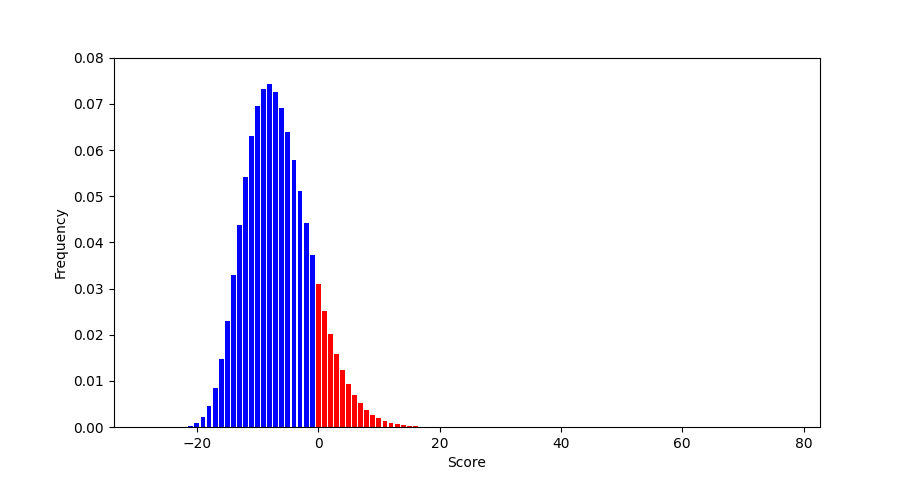
\includegraphics[scale=0.6]{graphics/distribution.png}
\end{center}
\caption{Example of score distribution \(h_7\) between uniformly
distributed \Qgram{7}. Blue denotes portion of the distribution where
\(\sigma < 0\). Red denotes portion of the distribution where \(\sigma \geq
0\).}
\label{fig:distrbution}
\end{figure}
Figure~\ref{fig:distrbution} visualizes an exemplary score distribution
between uniformly distributed \Qgram{7}. The red portion in the right
tail describes the probability \(\mathcal{P}(\sigma \geq 0)\), which could
be generally quantified to:
\begin{align}
\mathcal{P}(\sigma \geq k) = \sum_{i = k}^\infty h_q(i)
\end{align}
The average \Qgram{q} list length \(l\) could be normalized to
probability:
\begin{align}
p = \frac{l}{|\mathcal{A}|^q}
\end{align}
Therefore the approximation would be ideally in continuous distribution an
exact value:
\begin{align}
p = \mathcal{P}(\sigma \geq k)
\end{align}
or in discrete distribution, a value between two discrete values:
\begin{align}
\mathcal{P}(\sigma \geq k) \leq p < \mathcal{P}(\sigma \geq
k-1)\label{eq:distribution}
\end{align}
The idea of the algorithm is to approximate a \(q\times q\) score
distribution. Then the distribution can be iterated from the right tail to
calculate \(\mathcal{P}(\sigma \geq k)\), where \(k\) is the current score
threshold. The iteration can be stopped when Equation~\ref{eq:distribution}
is satisfied.
The \(q\times q\) score distribution can be approximated recursively
through convolution:
\begin{align}
h_{q}(x) = \sum_{y\in\mathcal{Z}} h_{q-1}(y)h_1(x-y)
\label{equation:convolution}
\end{align}
It is important to note that \(h_1\), the unigram score distribution,
depends on both character distribution collected from target sequence and
uniform character distribution, since the characters appeared in the
environment are independent from each other.
\textbf{Integrating context:} The above strategy treats single character as
independent and therefore loses its context in \Qgram{q}s. Another
approach could then be hashing the target sequences to collect \Qgram{q}
distribution, which is convenient since the work is done in the
preprocessing of target dabase. This approach is but often complicated by
large \(q\), since a \(q\times q\) score matrix must be computed, which
incur an additional penalty of \(O(|\mathcal{A}|^{2q})\), which is often
not feasible when \(q>4\). A middle ground is to divide the \Qgram{q}s
into two or three sub-\Qgram{q}s and collect their distribution
separately. These distributions can then in the end be convoluted together
to approximate the \Qgram{q} distribution. The extraction of threshold
\(k\) then follows the same approach in the context-free variant.
\Chapter{Implementation and Design}
\section{Design overview}
The program consists of seven main classes:
\begin{enumerate}
\item Seed readers convert seed into binary representation, computing its
span and weight. To further process seed, two variants are created:
\begin{enumerate}
\item Target reader divides seeds into blocks of shorter \Qgram{q}s as
input for recursive hashing function.
\item Query reader divides seeds into blocks of short segments, sorts query
sequences and uses sorted \Qgram{q} encoder to linearly encode the
resulted sorted \Qgram{q}s.
\end{enumerate}
\item A recursive hash engine to collect every \Qgram{q} hashes from
target sequences and package them.
\item A sorted \Qgram{q} index table to index every sorted \Qgram{q} of
given
scoring function and \(q\).
\item Sorted \Qgram{q} encoder creates a table to help linearly encode
sorted \Qgram{q}s.
\item A class to approximate an appropriate threshold given target sequence
data.
\item A score matrix to cache all scores between sorted \Qgram{q}s and
unsorted \Qgram{q}s.
\item An environment constructor gets sorted \Qgram{q} codes from the
query seed reader, uses them to call individual scores from the score
matrices and generates a Cartesian product from the environments.
\end{enumerate}
In Figure~\ref{fig:classes}, the relationship and dataflow between the
classes are outlined. Since the implementation of the recursive hashing of
target sequences is straightforward and doesn't diverge much from
pseudocode, the section below focuses mainly on the processing of query
sequences.
\begin{figure}[t]
\begin{center}
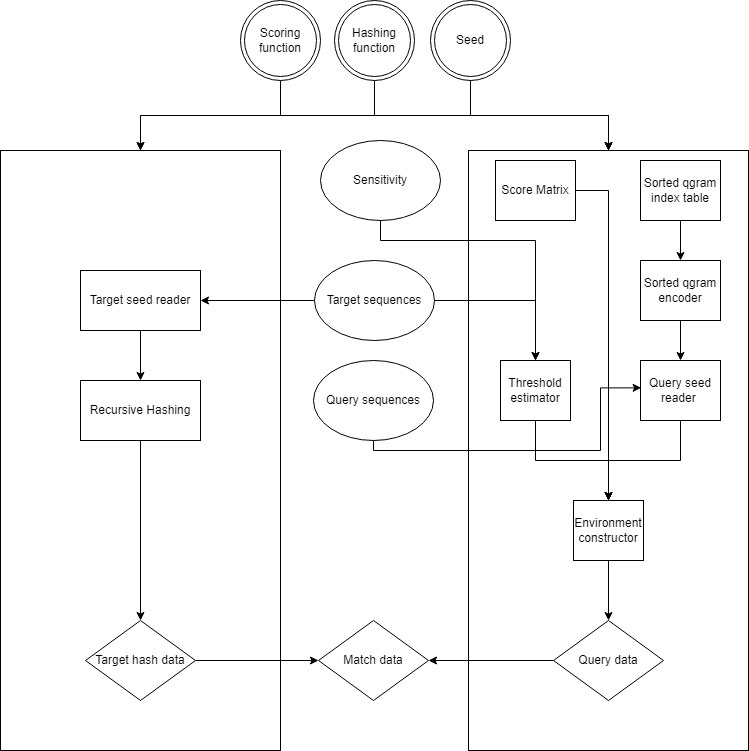
\includegraphics[scale=0.5]{graphics/Class_Diagram.png}
\end{center}
\caption{Relationship between the main classes and inputs}
\label{fig:classes}
\end{figure}
\section{Input}
At compile time, the program takes in a scoring function, which in the
context of protein sequences could be a BLOSUM or PAM matrix, a spaced seed
and a recursive hashing function. The scoring function should detail the
relevant alphabet, the transformer function, which encodes every character
in the alphabet to its corresponding rank, and a matrix of scores between
every pairs of characters. Internally, the spaced seed is initially
represented as a numeric constant, which during computation will be
transcoded into a bitset. The span of the seed can then be computed
according to the position of the first 1 in the bitset and also the seed
weight can be calculated by counting 1s.
At run time the program takes in two sequence databases in FASTA format.
Any data error, for example empty file or wrong data format will
automatically lead to termination of the program and an error message will
be logged. Additionally, the sensitivity of the program can be adjusted.
To further assist in expansion, some fixed parameters, e.g.\ maximum
sub-\Qgram{q} length are defined as preprocessor constants.
\section{Compile time computation}
Figure~\ref{fig:classes} shows that some classes/tables can be evaluated at
compile time. Each seed gets transcoded and its weight and span can be
precomputed and therefore, the two seed readers and their schematics can be
predetermined. The two index tables for sorted/unsorted digrams/trigrams
take in only scoring function as parameter and therefore, can be wholely
precomputed. Since the linear encoding table LE (see
Algorithm~\ref{code:linearEncodingTable}) based solely on the sorted
digrams/trigrams index table, it also can be evaluated at compilation.
\section{Run time computation}
At run time, firstly the target and query database gets encoded using the
transformer function. Using the target seed reader, the target sequences
can then be hashed in linear \(O(nb)\) time and the hashes are packaged as
byte units and saved in a contiguous container (i.e.\ array or vector).
In the processing of query sequences, firstly the \Qgram{2} and \Qgram{3}
score matrices \(\Scoretablename\) can be evaluated using the index tables
from sorted and unsorted \Qgram{q}s according to
Equation~\ref{equation:sequenceScore}. The result then can then be stored
as a pair of score and unsorted \Qgram{q} code and sorted after score
value for further use. Thereafter, an appropriate threshold is evaluated
using the target sequences and an user-provided sensitivity. Using the
score matrices and the threshold, the program enters the step of \Qgram{q}
generation using the Cartesian product.
\subsubsection{Local composition bias correction}
In the implementation of MMseqs2, a mechanism to evaluate the surrounding
of current position while iterating the query sequences is introduced. The
idea of this mechanism is to adjust the threshold of the \Qgram{q}
environment in response to regions where local composition varies
considerably from the background distribution. Without adjusting, these low
regions can lead to biases in the prefiltering result. This correction of
the threshold can be summarized as follow:
\begin{align}
\Delta \sigma_i(u[i]) =
\sum_{a=1}^{|\mathcal{A}|}f(a)\sigma(a,u[i])-\frac{1}{2d}\sum_{j=i-d,j\neq
i}^{i+d}\sigma (u[i],u[j])
\end{align}
where \(u\) is the query sequence, \(i\) the current residue on the
sequence and \(f(a)\) the background frequency of residue \(a\).
The minuend is a representation of the expected score resulting from the
background distribution, which can be precomputed when the target data is
read. The subtrahend involves the current region in the query sequence and
introduces a parameter \(d\) for the radius of the region, defined in
MMseqs2 as a constant 20.
The corrected score between a query \Qgram{q} \(u\) and its generated
\Qgram{q} \(v\) can then be computed as the sum of the pairwise amino acid
score and the score correction.
\begin{align}
\sigma_c(u,v) = \sigma (u,v) + \sum_{i=0}^{q-1} \sigma_i(u[i])
\end{align}
In the implementation, this correction is instead subtracted from the
threshold at the beginning of the computation.
\begin{align}
\sigma_c(u,v) = \sigma (u,v) + \sum_{i=0}^{q-1} \sigma_i(u[i]) \geq k
\Leftrightarrow \sigma (u,v) \geq k - \sum_{i=0}^{q-1} \sigma_i(u[i]) =
k_{c}
\end{align}
\subsubsection{Turning Wheel Mechanism}
An issue in enumerating the Cartesian product is the possible difference in
number of loops (e.g.\ 2 loops for seed weight 4-6, 3 loops for seed weight
7). To resolve this problem and allow easy expansion to greater seed
weight, a flexible loop structure is designed, where an array containing
the loop indexes is created. The earliest entry of the array holds the
outermost loop index and the later an entry is, the more inner the loop
index the entry holds. By iterating through only the innermost loop and
only adjusting the outer loop indexes as needed, the scheme can account for
any number of loops.
The formulation of the loop structure, is outlined in the
pseudocode~\ref{code:turningWheel}.
\begin{algorithm}[t]
\caption{Turning Wheel Mechanism}
\label{code:turningWheel}
\begin{tabular}{@{}l@{~}l}
\textbf{Input:}&number of loops \(n\)\\
&loop data vector \(v_0\), \(v_1\), ..., \(v_{n-1}\)\\
&threshold \(k\)\\
&function \(\mathsf{createQgram}\)\\
&function \(\mathsf{getScore}\)\\
&function \(\mathsf{getCode}\)
\end{tabular}
\begin{algorithmic}
\State \(\Loopid \gets n-1\)
\State \(\Wheel \gets [0]\times n\)
\State \(\Score \gets \mathsf{getScore}(\Wheel)\)
\If{\(\Score < k\)} \Comment{Current data vectors not viable. Early
Termination.}
\State return
\Else \Comment{First loop iteration}
\State \(\Code \gets \mathsf{getCode}(\Wheel)\)
\State \(\mathsf{createQgram}(\Code)\)
\EndIf
\While{True}
\State \(\Wheel[\Loopid]\gets \Wheel[\Loopid]+1\)
\If{\(\Wheel[\Loopid] \geq \text{len}(v_{\Loopid})\)}\Comment{End of loop}
\State \(\Wheel[\Loopid] \gets 0\)
\If{\(\Loopid = 0\)}\Comment{No longer viable in outermost loop}
\State break
\EndIf
\State \(\Loopid\gets \Loopid-1\)
\Else
\State \(\Score \gets \mathsf{getScore}(\Wheel)\)
\If{\(\Score \geq k\)}\Comment{Viable \Qgram{q} found}
\State \(\Code \gets \mathsf{getCode}(\Wheel)\)
\State \(\mathsf{createQgram}(\Code)\)
\Else \Comment{No viable \Qgram{q} found, end current loop}
\State \(\Wheel[\Loopid]\gets \text{len}(v_{\Loopid})\)
\EndIf
\If{\(\Loopid \neq n-1\)}\Comment{Reset to innermost loop}
\State \(\Loopid \gets n-1\)
\EndIf
\EndIf
\EndWhile
\end{algorithmic}
\end{algorithm}
\subsubsection{SIMD}
SIMD (Single-Instruction Multiple-Data) is a group of instructions allowing
vectorized, parallel data processing. Instead of processing data
sequentially, they are capable of defining wide registers, commonly 128-bit
or 256-bit, packaging data in those registers and process data in parallel.
The key to the shuffle using SIMD is the instruction
\(\mathsf{\_\_mm\_shuffle\_epi8}\), which is available on platforms
supporting
SSSE3 instruction sets or the equivalent \(\mathsf{vqtbl1q\_u8}\) on ARM
platform. Both instructions take in two 128-bit (equivalent to 16-byte)
vectors.
In order to comply with the instructions, both the \Qgram{q} and the
inverse
permutation get padded internally to 16-byte. First vector holds the data,
in
this case the \Qgram{q}, and the second the information on how the data get
shuffled, in this case the inverse permutation.
\begin{figure}[t]
\begin{center}
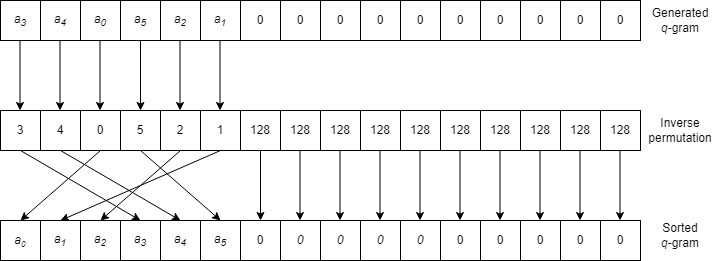
\includegraphics[scale=0.6]{graphics/SIMD.png}
\end{center}
\caption{Schematics of SIMD instruction \_\_mm\_shuffle\_epi8}
\label{fig:simd}
\end{figure}
A schematic is visualized in Figure~\ref{fig:simd}. The right padded
section of the inverse permutation is filled with integer 128 to signal the
instruction to not shuffle and to simply pad the resulted vector with 0.
\section{Merging target and query data}
After being collected, the hashed data from the target and query sequences
are packaged as byte units, prioritizing hash values. They then get sorted
individually using radix sort (see GTTL~\cite{gttl}), resulting in two data
vectors
sorted by hash values which would then be merged value by value, skipping
through unmatching blocks.
\begin{algorithm}[t]
\caption{Merging query and target data}
\label{code:merging_data}
\begin{tabular}{@{}l@{~}l}
\textbf{Input:}&query data \(\Query\)\\
&target data \(\Target\)\\
&function \(\mathsf{CreateMatch}\)
\end{tabular}
\begin{algorithmic}
\State \(\TargetIdx \gets 0\)
\State \(\QueryIdx \gets 0\)
\While{\(\TargetIdx \neq \Target.\End\) \(\land\) \(\QueryIdx \neq
\Query.\End\)}
\State \(\HashValue_t \gets \Target[\TargetIdx].\HashValue\)
\State \(\HashValue_q \gets \Query[\QueryIdx].\HashValue\)
\If{\(\HashValue_t < \HashValue_q\)} \Comment{Skipping on target vector}
\While{\(\Target[\TargetIdx].\HashValue = \HashValue_t\)}
\State \(\TargetIdx\gets\TargetIdx+1\)
\EndWhile
\Else
\If{\(\HashValue_t > \HashValue_q\)} \Comment{Skipping on query vector}
\While{\(\Query[\QueryIdx].\HashValue = \HashValue_q\)}
\State \(\QueryIdx\gets\QueryIdx+1\)
\EndWhile
\Else \Comment{Match found}
\State \(\TBlockEnd = \TargetIdx\)
\While{\(\Target[\TBlockEnd] = \HashValue_t\)}
\State \(\TBlockEnd\gets\TBlockEnd+1\)
\EndWhile
\State \(\QBlockEnd = \QueryIdx\)
\While{\(\Query[\QBlockEnd] = \HashValue_q\)}
\State \(\QBlockEnd\gets\QBlockEnd+1\)
\EndWhile
\State
\(\mathsf{CreateMatch}([\TargetIdx,\TBlockEnd),[\QueryIdx,\QBlockEnd))\)
\State \(\TargetIdx\gets\TBlockEnd\)
\State \(\QueryIdx\gets\QBlockEnd\)
\EndIf
\EndIf
\EndWhile
\end{algorithmic}
\end{algorithm}
The merging process results in a vector of matches, represented again as
byte units, containing respectively the sequence number of the match on the
target, on the query, the diagonal number (difference between the target
and query sequence position), and the query sequence position. These
quartets are again sorted with radix sort to prepare for ungapped alignment
stage.
\Chapter{Benchmark and Performance}
Separate modular benchmarks were carried out for the processing of target
sequences, threshold estimation and similar \Qgram{q} generation. All
measurements were performed using C++ on an Intel CPU i5-\numprint{10300}H
2.5~GHz
with 8~GB DDR4 running Ubuntu on a SSD. The program was compiled with g++
11.3.0.
The test dataset composed of a target database from MMseqs2 and a query
database created as a difference set from MMseqs2 queryset against the
target database. Some statistics on these datasets are summarized below in
Table~\ref{tab:datasets}. Table~\ref{tab:seeds} outlines the spaced seeds
used in testing, which are taken from MMseqs2.
\section{Processing target sequences}
Testing from Figure~\ref{fig:target_hashing} showed that the direct
extraction of \Qgram{q}s generally has a better run time. Recursive hashing
only presented better performance when the spaced seeds have no block or
with 1 block with high weight. The reason could be repeated lookup of
character to remove/add causing cache-miss, slowing the computation.
\begin{figure}[t]
\begin{center}
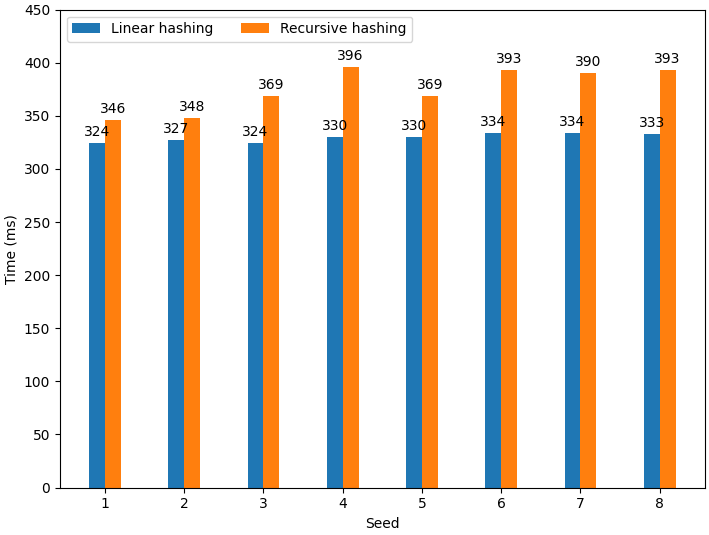
\includegraphics[scale=0.45]{graphics/target_hashing.png}
\end{center}
\caption{Performance of two hashing functions}
\label{fig:target_hashing}
\end{figure}
\section{Determining threshold}
In order to test the accuracy of the threshold estimation, measurements
were firstly carried out on MMseqs2 with default seed.
\begin{figure}
\centering
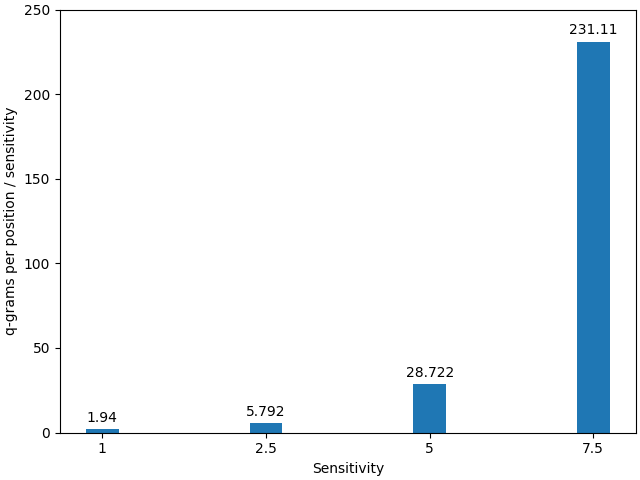
\includegraphics[scale=0.6]{graphics/mmseqs2_sensitivity.png}
\caption{Ratio of number of generated \Qgram{q}s using MMseqs2 approach
vs. expected}
\label{fig:mmseqssens}
\end{figure}
The test shows that MMseqs2 often overgenerated \Qgram{q}s, with the worst
case creating 231.11~\% more than expected. Both of the approaches,
context-free and context-sensitive, were tested with the dividing scheme in
context-sensitive approach reused from the \Qgram{q} generation algorithm.
For each test, the total number of \Qgram{q}s generated is averaged and
then compared to the expected list length per position and MMseqs2 result.
\begin{figure}
\centering
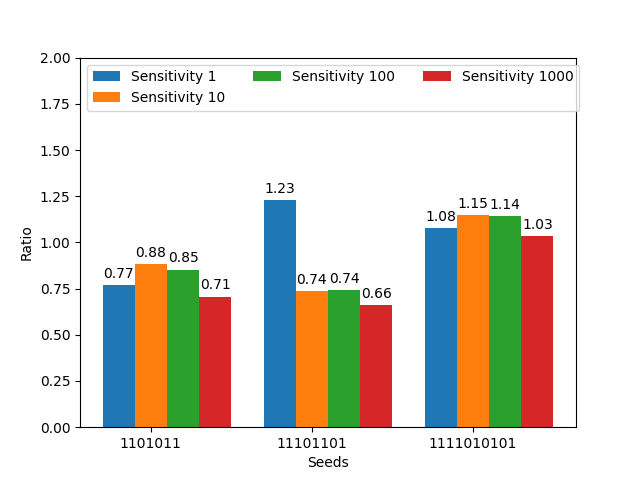
\includegraphics[scale=0.6]{graphics/threshold_contextfree.png}
\caption{Ratio of number of generated \Qgram{q}s using context-free
approach vs. expected}
\label{fig:numctxfree}
\end{figure}
\begin{figure}
\centering
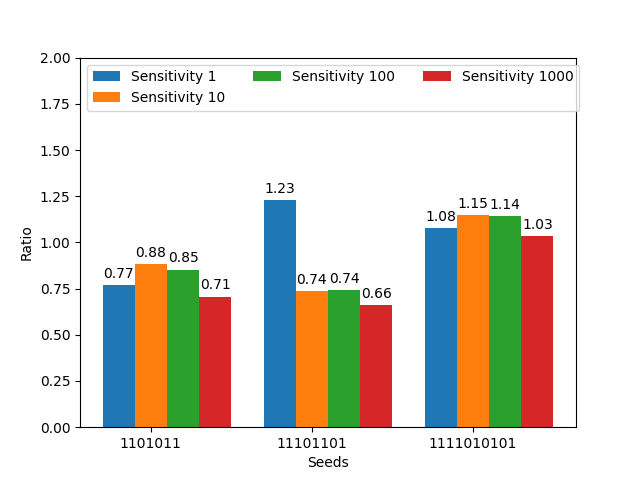
\includegraphics[scale=0.6]{graphics/threshold_contextsens.png}
\caption{Ratio of number of generated \Qgram{q}s using context-free
approach vs. expected}
\label{fig:numctxsens}
\end{figure}
The benchmarks of context-free (Figure~\ref{fig:numctxfree}) and
context-sensitive approach (Figure~\ref{fig:numctxsens}) both show better
control compared to MMseqs2 and the resulted list lengths are relatively
close to the expected value. The thresholds created by this approach show
to be a good upper bounds for the \(k\)-environment in lower \(q\), where
only sensitivity of 1 in the seed weight 6 crosses the expected ammount. In
higher seed weight, both approaches serve well as an approximation, where
only a maximum of 15~\% more \Qgram{q}s were generated compared to
expected value. In order to discern the usage of each approach,the run time
of each method is investigated further in Figure~\ref{fig:sens_runtime}:
\begin{figure}
\centering
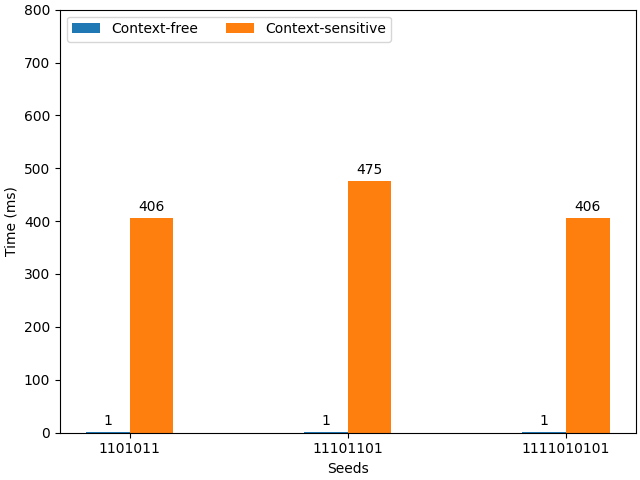
\includegraphics[scale=0.6]{graphics/speed_threshold.png}
\caption{Run time comparison of context-free vs. context-sensitive
approach}
\label{fig:sens_runtime}
\end{figure}
\AVTcomment{I'm looking to make a stacked bar chart with annotation on each
bar as legend for each smaller step, e.g.\ for context-sensitive it would
be
extracting frequency of sub-\Qgram{q} and creating histogram.}
The context-free approach shows to take very little time, almost
instanteneous.
Coupled with the very good estimation of the threshold it proves to be an
universal on-the-fly solution. The context-sensitive approach takes a lot
more
time, average around 0.5~s to create a threshold (compensated for creation
of
unsorted-unsorted \Qgram{q} score matrices, see
Section~\ref{section:scorematrix}),since it incurs a \(O(|\Alpha|^{2q})\)
time to build histogram. Therefore this approach should be used only on
high
sensitivity, where long computation time is expected, or cached in the
preprocessing of target sequences.
It is important to note that since the approximation of the threshold \(k\)
doesn't take local score correction into account, all of the above
measurements are without local score correction. In
Figure~\ref{fig:compbias} are some benchmarks with correction of varying
degree, showcasing how the average list length is impacted. The result
shows that the average \Qgram{q} list can vary strongly and unpredictably
under usage of local composition bias score correction, where if the scale
of the correction is from 0.75~-~1, the resulted number can be as few as 5
times or as many as 48 times more than expected. The proper scaling of the
factor remains to be investigated further.
\begin{figure}
\centering
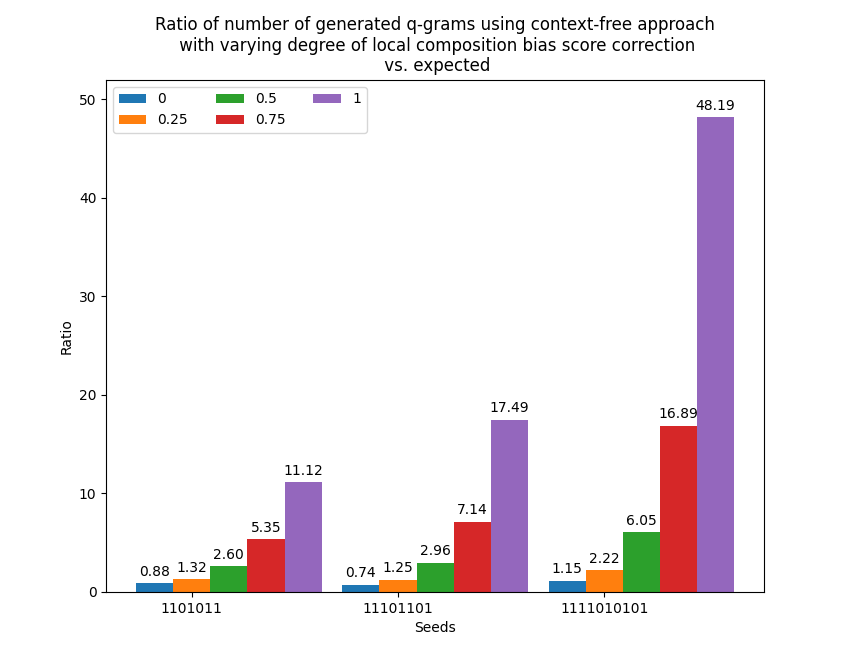
\includegraphics[scale=0.6]{graphics/comp_bias.png}
\caption{Influence of local composition bias score correction on average
\Qgram{q} list length. The original estimation on \Qgram{q} list length
was 10.}
\label{fig:compbias}
\end{figure}
\section{Generating \Qgram{q}s}
In order to test the efficiency of the \Qgram{q} list generation, the
original workflow in MMseqs2 was replicated and tested against the new
algorithm. This workflow, along with both variants of the new algorithm,
with and without SIMD implementation, was measured in
Figure~\ref{fig:genw5}, \ref{fig:genw6} and \ref{fig:genw7} for different
seed weights.
\begin{figure}
\centering
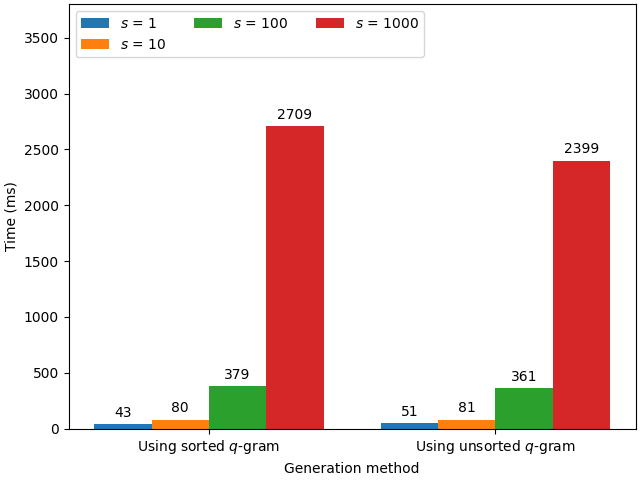
\includegraphics[scale=0.6]{graphics/gen_w5.png}
\caption{Time measured in miliseconds to generate \Qgram{q}s with
different sensitivities using seed \numprint{1101011}}
\label{fig:genw5}
\end{figure}
\begin{figure}
\centering
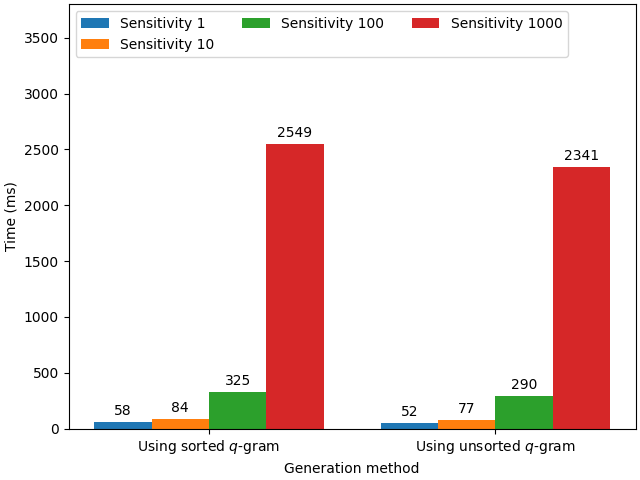
\includegraphics[scale=0.6]{graphics/gen_w6.png}
\caption{Time measured in miliseconds to generate \Qgram{q}s with
different sensitivities using seed \numprint{11101101}}
\label{fig:genw6}
\end{figure}
\begin{figure}
\centering
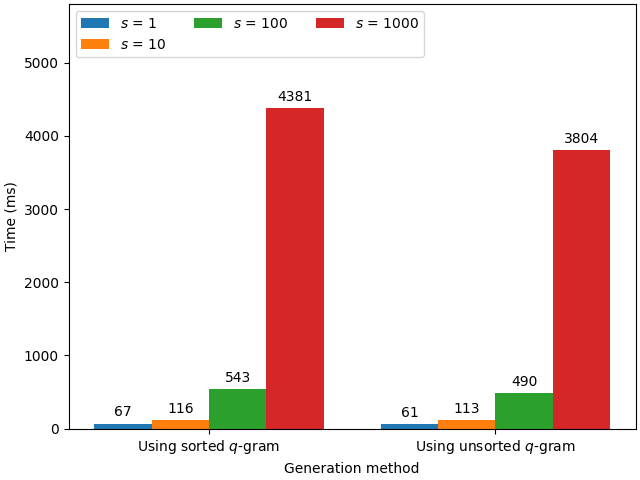
\includegraphics[scale=0.6]{graphics/gen_w7.png}
\caption{Time measured in miliseconds to generate \Qgram{q}s with
different sensitivities using seed \numprint{1111010101}}
\label{fig:genw7}
\end{figure}
The tests showed that the new algorithm has generally a 10~\% to 15~\%
performance loss compared to the MMseqs2 method. This is the overhead
caused by the sorting and reshuffled of \Qgram{q}. The tradeoff is the low
initial memory consumption, where only 36~MB of memory is consumed for the
score matrices instead of 200~MB. The SIMD function unfortunately shows to
have an negative impact on performance, which could be due to the SIMD
instruction not optimized for the large padded section. On average, the
program spends 18.2~ns to generate a \Qgram{5}, 18.3~ns to generate a
\Qgram{6} and 20.1~ns to generate a \Qgram{7}. This shows that the
\Qgram{q}
generation scales generally well with \(q\), where an additional loop in
creation of \Qgram{7} causing an increase of 10~\%. It could be reasoned
that the generation of \Qgram{8} and \Qgram{9} may follow the same trend,
which coupled with the new approach in estimating threshold could lead to
an expansion of seed weight (see Section~\ref{section:expand}).
\section{General Performance}
In this section, the overall run time of the whole program is profiled to
find hotspots and to figure the scalability of the system. The program will
be run with the most optimized settings, meaning context-free threshold
approximation and \Qgram{q} generation using sorted method. In Figure, the
recorded time in each step of the program is visualized.
\begin{figure}
\centering
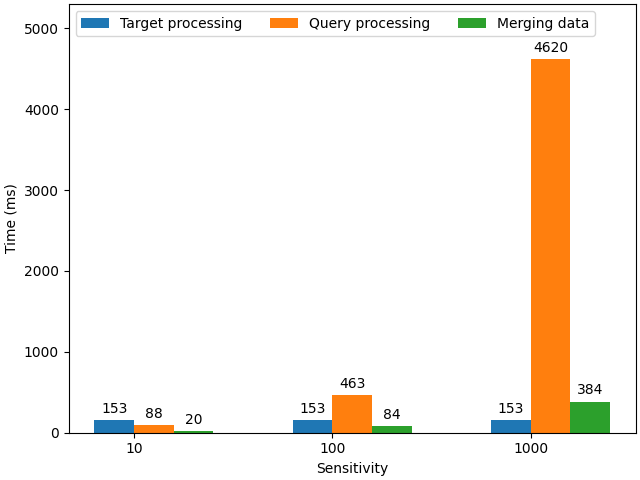
\includegraphics[scale=0.6]{graphics/program_w6.png}
\caption{Run time of different phases in the program, measured in
miliseconds,
using seed \numprint{11101101}, sensitivity 10, 100 and \numprint{1000}}
\label{fig:program_w6}
\end{figure}
\begin{figure}
\centering
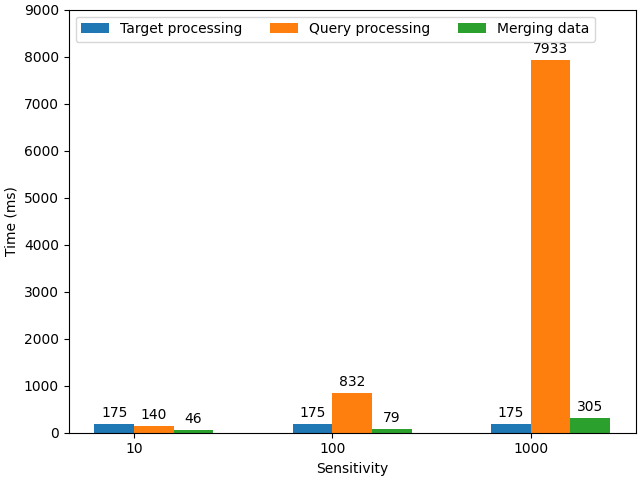
\includegraphics[scale=0.6]{graphics/program_w7.png}
\caption{Run time of different phases in the program, measured in
miliseconds,
using seed \numprint{1111010101}, sensitivity 10, 100 and \numprint{1000}}
\label{fig:program_w7}
\end{figure}
\AVTcomment{Same as last comment}
The test showed that the run time of processing target data is generally
negligible. The processing of match data could be more significant,
reaching
0.4~s in testing but still scales much better than \Qgram{q} generation
phase.
This means that the hotspot of the program lies in the \Qgram{q} generation
phase, specifically in the Cartesian product formation and in lesser
manner,
the radix sort of \Qgram{q} data. In the most heavy measurement, the
\Qgram{q}
generation phase still takes twice as long as the sorting after.
\Chapter{Discussion \& Future improvements}
\section{Features}
The new workflow was created with expandability in mind, therefore a lot of
the calculation allows for greater seed size and even greater sub-\Qgram{q}
size. A few of MMseqs2 features were also recreated, namely the ability to
scale local composition bias correction and sensitivity manually. The
design of the program also prioritizes flexibility, in that every
calculation option, ranging from MMseqs2 mode vs new sorted \Qgram{q}
method mode and both context-free and context-sensitive approach can be
changed on-the-fly without recompilation.
The program was intended to be a testing environment only, therefore custom
workflows in MMseqs2 were not recreated, namely the stepwise sensitive
search.
\section{Possibility of expanding seed\label{section:expand}}
Earlier it was shown that the run time of \Qgram{q} generation scales
almost constantly to seed, therefore some testing was created to test for
seeds of weight 8 and 9:
\AVTcomment{Waiting for BytesUnit fix}
\section{Compile-time calculation of
score matrices\label{section:scorematrix}}
Even though the class diagram in Figure~\ref{fig:classes} shows that it's
possible to compute the score matrix in compile time, since it only depends
on the two index tables of sorted/unsorted \Qgram{q}s, the implementation
decides to create the table in run time instead. The reason largely is due
to the high memory stack size requirements and lack of compile time sorting
algorithm. A manual compile time sorting implementation (i.e.\ quicksort)
would again demand more compile time instances. A separate benchmark in
Figure~\ref{fig:scorematrix} showed that this could incur a 0.6~s loss in
creating the sorted-unsorted \Qgram{3} score matrix or 3.3~s in creating
the unsorted-unsorted \Qgram{3} score matrix at the start of the
computation.
\begin{figure}
\centering
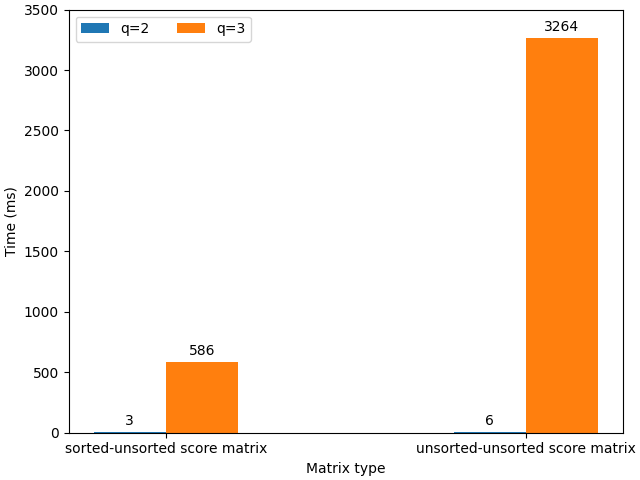
\includegraphics[scale=0.7]{graphics/scorematrix.png}
\caption{Time measured in miliseconds to generate \(q\times q\) score
matrix}
\label{fig:scorematrix}
\end{figure}
\section{Performance}
Even though the new workflow shows general improvements on performance, the
implementation still falls short compared to original MMseqs2 program,
especially in large \Qgram{q} list length.This shows that there is still
possible future optimization, particularly in loops. Another important
further improvent would be the ability to process the data in multithreads.
\Chapter{Conclusion}
In this paper, the prefiltering module of the MMseqs2 software suite was
examined and alternative optimization methods were tried and tested. A
possible improvement in processing target sequences through recursive
hashing, although has a better time complexity in theory, was shown to not
be a major improvement, other than in edge cases of low block numbers. A
new method of estimating threshold for better estimation of number of
generated \Qgram{q}s was implemented and showed to be a better estimation
approach, both in low and high sensitivity. Finally, an optimized
branch-and-bound algorithm was introduced and presented a lower memory
consumption in tradeoff for marginal increase in run time, allowing future
expansion into larger seed size.
%%%%<
%bibliography
\newpage
\small
% change the name of the bib-file to get your own bibliography
\bibliographystyle{unsrt}
\bibliography{template}
\normalsize
%%%%END{fold}
%%%%>
% appendix
\appendix
\noappendicestocpagenum
\addappheadtotoc
\Chapter{Some additional method descriptions}
\begin{table}
\begin{center}
\begin{tabular}{c|c|c|c}
Dataset & Number of sequences & Maximum Sequence Length & Minimum Sequence
Length\\
\hline
QUERY\_DIFF & 426 & \numprint{4291} & 8\\
TARGET & \numprint{20000} & \numprint{8081} & 7\\
\end{tabular}
\caption{Datasets used in testing the modules\label{tab:datasets}}
\end{center}
\end{table}
\begin{table}
\begin{center}
\begin{tabular}{c|c|c|c|c}
Nr & Seed & Span & Weight & Number of Blocks\\
\hline
1& \numprint{11101} & 5 & 4 & 2\\
2& \numprint{111011} & 6 & 5 & 2\\
3& \numprint{1101011} & 7 & 5 & 3\\
4& \numprint{110010000101} & 12 & 5 & 4\\
5& \numprint{11101101} & 8 & 6 & 3\\
6& \numprint{1101010011} & 10 & 6 & 4\\
7& \numprint{1111010101} & 10 & 7 & 5\\
8& \numprint{11010110011} & 11 & 7 & 4\\
\end{tabular}
\caption{Seeds used in testing\label{tab:seeds}}
\end{center}
\end{table}
\Chapter{Some Additional Data}
%%%%<
\Assertion
\end{document}
